\chapter{Espacios topológicos}
\label{cha:espacios_topologicos}

\section{Conjuntos abiertos}
\label{sec:conjuntos_abiertos}
\begin{defi}[Espacio Topológico]
Sea $X$ un conjunto y $\mathcal{T} \subset \mathcal{P}\left( X \right)$ una colección de subconjuntos del mismo, decimos que $\mathcal{T}$ es una \textbf{topología} de $X$ si y sólo si:
\begin{enumerate}
    \item $\emptyset, X \in \mathcal{T}$ 
    \item $\bigcup_{i \in I} U_i \in \mathcal{T}$ donde $U_i \in \mathcal{T}$
    \item $\bigcap_{i=1}^n U_i \in \mathcal{T}$ donde $U_i \in \mathcal{T}$
\end{enumerate}
y denotamos por \textbf{espacio topolócio} al par $\left( X, \mathcal{T} \right)$. A los elementos de $X$ los llamaremos puntos y a los elementos de $\mathcal{T}$ los llamaremos abiertos.
\end{defi}

\begin{ej}
\begin{enumerate}
    \item \label{ejemplos_topologia:first} $\mathcal{T} = \{\emptyset, X\}$ es la topología \textbf{trivial}, que está contenida en cualquier otra topología.
    \item $\mathcal{T} = P\left( X \right)$ es la topología \textbf{discreta}, que contiene a cualquier\footnote{En parte porque si los puntos $\{x\} \in \mathcal{T}$ son abiertos, entonces cualquier conjunto $A = \bigcup_{x \in A} \{x\}$ es abierto.} otra topología.
    \item $\mathbb{R}^n$ junto con las bolas euclídeas es la topología habitual que utilizamos.
    \item Cualquier distancia $d(x,y)$ define una topología a través de sus bolas abiertas, igual que definíamos la usual en $\mathbb{R}^n$, de hecho, se puede demostrar sin mayor dificultad (y tal y como se ve en el dibujo) que todas las normas $p$ en $\mathbb{R}^n$ definen bolas que contienen y están contenidas en las restantes. En consecuencia, si la definición de abierto usual se hacía a través de bolas redondas y hemos visto que estas contienen a bolas cuadradas o romboidales, también se tiene que es abierto cuadrado o romboidal y el recíproco por los contenidos en ambos lados.
    %TODO: esto debería hacerse con el entorno figure para que la anotación de abajo sea un caption
    \begin{center}
        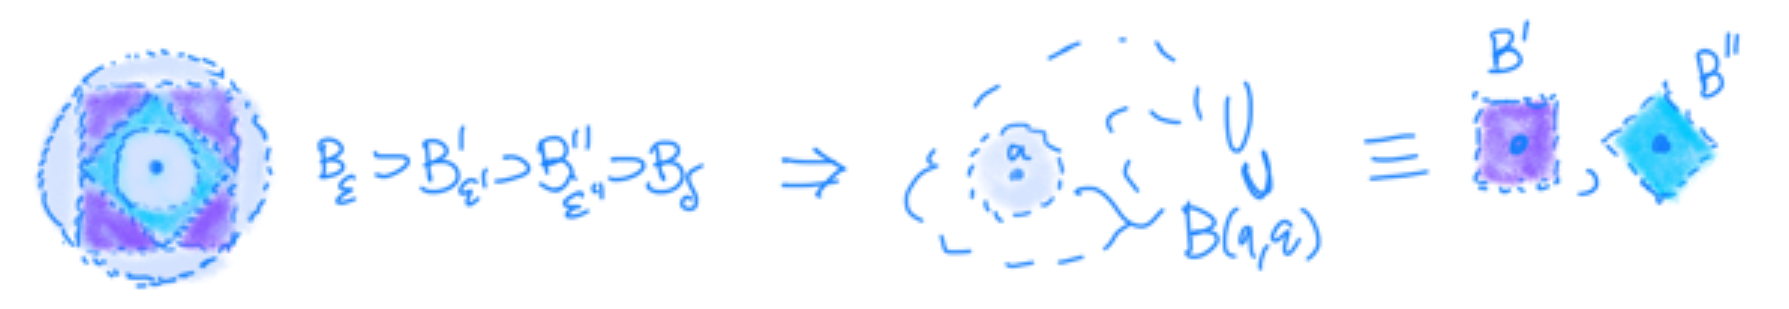
\includegraphics[scale=0.2]{images/topologia_metricas}  

        \textit{El dibujo representa distintas distancias\footnote{Procedentes de \textit{normas}.} en $\mathbb{R}^n$, pero todas definen la misma topología.} 
    \end{center}
    Es decir, cambiar de norma igual cambia la noción de distancia en $\mathbb{R}^n$, ¡pero no la topología asociada! Sigue siendo la topología usual de $\mathbb{R}^n$.
    
    \item En general, cuando queramos ver resultados que no son ciertos pondremos un contraejemplo donde no se cumpla. Para poder hacer esto, tenemos que disponer de muchos y muy variados ejemplos de topologías poco usuales, como por ejemplo, la topología ``del punto'':
    $$
    \mbox{Fijado } a \in X : \mathcal{T}_a := \{U \subset X: a \in U\} \cup \{\emptyset\} 
    $$
    En esta topología, el punto $\{a\}$ y todos los pares $\{a, x\}$ son abiertos y, aunque puede parecer igual a la discreta, no lo es. Hay que fijarse en que los abiertos de esta topología son los que contienen al punto, no todos los puntos en general. De este modo, $\{x\}\notin \mathcal{T}$, pero $\{a,x_1, x_2, \ldots\}\in \mathcal{T}$.
\end{enumerate}
\end{ej}

\begin{defi}[Entorno]
Sea $(X, \mathcal{T})$ un espacio topológico y $x\in X$ un punto del mismo, definimos un \textbf{entorno\footnote{Cuando el abierto que contiene al punto es el propio entorno o, dicho de otra manera, el entorno de $x$ es un abierto de la topología, decimos que es un entorno \textit{abierto} de $x$.} de $x$} como un conjunto $V^x$ que contiene un abierto $U$ que contiene al punto.
\end{defi}

\begin{prop}[Caracterización de abierto]
Sea $(X, \mathcal{T})$ un espacio topológico y $W \subset X$ un subconjunto de puntos, este es abierto si y sólo si es entorno de todos sus puntos.
\end{prop}
\begin{demo}
La implicación de izquierda a derecha es trivial, pues todo conjunto se contiene a sí mismo y, como el conjunto es abierto, contiene a un abierto que contiene al punto, es decir, es entorno de cualquiera de sus puntos.

Para probar el recíproco, si un subconjunto $W\subset X$ es entorno de todos sus puntos, entonces para cada $x$ del conjunto existe un $U^x\subset W$ que contiene a $x$. Por tanto, podemos expresar $W$ como unión arbitraria de todos estos abiertos, es decir, $W = \bigcup_{x\in W} U^x$ y, por ser topología, la unión arbitraria de abiertos es abierta.
\end{demo}

\begin{prop}
Sea $(X,\mathcal{T})$ un espacio topológico y $V_1^x$ y $V_2^x$ dos entornos de un punto $x\in X$, entonces la intersección $V^x := V_1^x\cap V_2^x$ es entorno de $x$.
\end{prop}
\begin{demo}
Por definición de entornos, existen dos abiertos $U_1^x\subset V_1^x$ y $U_2^x\subset V_2^x$ que contienen a $x$. Por la definición de topología, la intersección finita $U^x := U_1^x\cap U_2^x$ es un abierto de la topología y vemos que $U^x \subset V^x$, luego $V^x$ contiene a un abierto que contiene al punto, es decir, es entorno.
\end{demo}

\begin{defi}[Punto interior]
Sea $(X,\mathcal{T})$ un espacio topológico y $A \subset X$ un subconjunto de puntos, decimos que un punto $x\in X$ es \textbf{punto interior de $A$} si y sólo si $A$ es entorno de $x$.
$$
x\in \inter_X(A) \Leftrightarrow \exists U^{\text{ab.}} \subset A : x \in U
$$
Al conjunto de puntos interiores lo llamamos \textbf{interior de $A$} y se denota por $\inter_X \left( A \right)$ o $\mathring{A}$.
\end{defi}
%TODO: Fix imagen
\begin{center}
    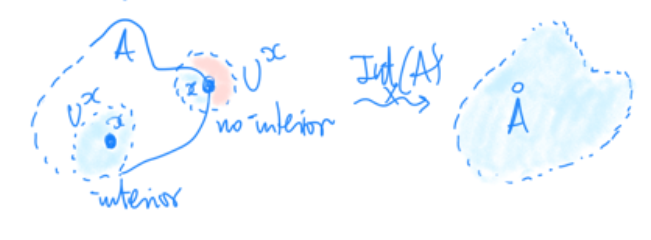
\includegraphics[scale=0.4]{images/def_interior} 
\end{center}

\begin{prop}
Sea $A\subset X$ un subconjunto de puntos, entonces:
\begin{itemize}
\item $\mathring{A}$ es el mayor abierto en $A$ o lo que es lo mismo $ \mathring{A} = \bigcup_{U \subset A} U$.
\item $A$ abierto si y sólo si todos sus puntos son interiores, es decir, $A = \mathring{A}$
\item $A$ es abierto si y sólo si es entorno de todos sus puntos.
\end{itemize}
\end{prop}
\begin{demo}
\begin{enumerate}
    \item Si $x\in \mathring{A}$, entonces $\exists U \subset A : x\in U \Rightarrow x\in \bigcup_{U\subset A}U$, pero es que si $x\in U$ para algún $U\subset A$, por definición es interior de $A$, luego $x\in \mathring{A}$.
   
   Como $\mathring{A}$ es unión de abiertos, la definición de topología nos asegura que será un abierto y además es el más grande de todos porque cualquier otro está contenido en él por ser la unión de todos los abiertos.   
   \item El contenido $\mathring{A}\subset A$ se tiene siempre, puesto que $x\in \mathring{A}\Leftrightarrow \exists U \subset A : x\in U \subset A \Rightarrow x\in A$ (dicho de otra forma, los puntos interiores de $A$ son aquellos para los cuales $A$ es entorno y como un entorno contiene al punto se tiene trivialmente).
   
   De esta manera, si $A$ es abierto, como $\mathring{A}$ es el mayor abierto de $A$, tiene que ser $\mathring{A} = A$ y si $\mathring{A} = A$, como $\mathring{A}$ es abierto, pues lo es $A$.
    
   \item Se tiene trivialmente de la implicación anterior. Cuando $A$ es abierto sabemos que todos los puntos son interiores y un punto es interior si y sólo si $A$ es entorno para él, luego es entorno para todos sus puntos.
   
   Recíprocamente, $A$ es entorno de todos sus puntos, entonces todos sus puntos están en el interior y $A = \mathring{A}$, lo que indica que es abierto.
\end{enumerate}
\end{demo}

\begin{ej}
\begin{enumerate}
    \item $\left( X, \mathcal{T}_{\text{trivial}} \right): A \neq X \Rightarrow A \not \supset X \Rightarrow \emptyset$ es el único abierto $\subset A \Rightarrow \mathring{A} = \emptyset$.

    \item En $\mathbb{R}^n$ con $\mathcal{T}_{\text{trivial}}$ ya lo sabemos bien:
    \[
    \inter\left( B\left[ a, \varepsilon \right] \right)  = B\left( a, \varepsilon \right);\ \mathring{\mathbb{Q}}^n = \emptyset;\ \mathring{\mathbb{Z}}^n = \emptyset
    \]
    \item Si $a \in X,\ \mathcal{T}_a : \mathring{\{a\}} = \{a\};\ x \neq a,\ \mathring{\{x\}} = \emptyset$.
\end{enumerate}
\end{ej}

\begin{coro}
\begin{enumerate}
    \item $A \subset B \Rightarrow \mathring{A} \subset \mathring{B}$.
    \item $\mathring{A} \cap \mathring{B} = \inter \left( A \cap B \right)$.
\end{enumerate}
\end{coro}
\begin{demo}
\begin{enumerate}
    \item La relación $A \subset B \Rightarrow \mathring{A} \subset A \subset B$ implica que, como $\mathring{A}$ es abierto y $\mathring{B}$ es la unión de todos los abiertos de $B$, $\mathring{A} \subset \mathring{B}$.
    \item En primer lugar, como $\mathring{A}\cap \mathring{B}$ es intersección de abiertos, entonces es abierto y está contenido en $A\cap B$, luego por ser $\inter(A\cap B) = \bigcup_{U\in A\cap B}U$ sabemos que $\mathring{A}\cap \mathring{B} \subset \inter(A\cap B)$.
    
	Recíprocamente, si $x\in \inter(A\cap B)$ existe un abierto $U \in A\cap B$ tal que $x\in U$. Por ser de la intersección, en particular también es abierto de cada conjunto, luego $x\in \mathring{A}$ y $x\in \mathring{B}$, es decir, $x\in \mathring{A}\cap \mathring{B}$.
\end{enumerate}
\end{demo}

\section{Conjuntos cerrados}%
\label{sec:conjuntos_cerrados}

\begin{defi}[Conjunto cerrado]
Sea $\left( X, \mathcal{T} \right)$ un espacio topológico, definimos un \textbf{conjunto cerrado} como $F \subset X : U = X \setminus F$ es abierto.
\end{defi}
\begin{obs}
A pesar de lo que pueda sugerir el lenguaje habitual, la definición cerrado NO significa ``no abierto'', hay conjuntos que no son ni abiertos ni cerrados.
    \begin{center}
        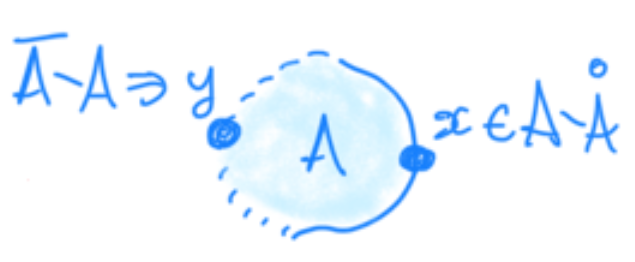
\includegraphics[scale=0.3]{images/def_cerrados} 
    \end{center}
y otros que son abiertos y cerrados simultáneamente, como son el vacío y el total.
\end{obs}

\begin{prop}
Sea $(X,\mathcal{T})$ un espacio topológico y denotando por $\mathcal{F}$ al conjunto de cerrados del espacio, entonces:
\begin{enumerate}
    \item $\emptyset, X \in \mathcal{F}$ 
    \item $\bigcap_{F \in \mathcal{F}} F \in \mathcal{F}$
    \item $\bigcup_{i=1}^n F_i \in \mathcal{F}$ donde $F_i \in \mathcal{F}$
\end{enumerate}
\end{prop}
\begin{demo}
\begin{itemize}
\item Trivial, porque el uno es el complementario del otro y ambos son abiertos.

\item Porque el complementario de la intersección $X\setminus \left(\bigcap_{F \in \mathcal{F}} F\right) = \bigcup_{F \in \mathcal{F}} \left( X \setminus F \right) = \bigcup_{F \in \mathcal{F}} U_F$ es abierto.

\item Porque el complementario de la unión $X\setminus \left(\bigcup_{i = 0}^n F_i\right) = \bigcap_{i=0}^n \left( X \setminus F_i\right) = \bigcap_{i=0}^n U_i$ es abierto.
\end{itemize}
\end{demo}

\begin{ej}
\begin{enumerate}
    \item En la topología trivial solo son cerrados $\emptyset$ y $X$ y en la discreta, todos los subconjuntos son cerrados.
    \item En $\mathbb{R}^n$ con la topología usual ya sabemos todos los ejemplos: $B\left[ a, \varepsilon \right] : \lVert x - a \rVert \le \varepsilon$.
    \item Si $\mathcal{T}_1 \subset \mathcal{T}_2$, todo cerrado de $\mathcal{T}_1$ es cerrado de $\mathcal{T}_2$, pues es cerrado por ser el complementario de un abierto y los abiertos de $\mathcal{T}_1$ también lo son el $\mathcal{T}_2$.
\end{enumerate}
\end{ej}

\begin{defi}[Adherencia]
Sea $A \subset X$ y $x\in X$ un punto, decimos que es \textbf{adherente a $A$} si y sólo si todos sus entornos intersecan con $A$.
$$
\adh_X\left( A \right) = \overline{A} := \{x \in X: \forall V^x \cap A \neq \emptyset\} \supset A
$$
al conjunto de puntos adherentes a $A$ lo llamamos su \textbf{adherencia}.
\end{defi}

\begin{obs}
La propia definición nos sugiere ciertas equivalencias útiles que se obtienen escribiendo de forma distinta lo que hemos definido:
\begin{itemize}
\item $X \setminus \overline{A} = \inter\left( X \setminus A \right)$
$$
x \in X \setminus \overline{A} \Leftrightarrow x \not\in \overline{A} \Leftrightarrow \exists U^x \cap A = \emptyset \Leftrightarrow \exists U^x \subset X \setminus A \Leftrightarrow x \in \inter\left( X \setminus A \right)
$$
\item $X \setminus \mathring{B} = \overline{X \setminus B}$
$$
x \not\in \mathring{B} \Leftrightarrow \nexists U^x \subset B \Leftrightarrow \forall U^x \cap \left( X \setminus B \right) \neq \emptyset \Leftrightarrow x \in \overline{X \setminus B}
$$
\end{itemize}
\end{obs}

\begin{prop}
Sea $A\subset X$ un subconjunto de puntos y denotando por $\overline{A}$ a su adherencia, entonces:
\begin{itemize}
\item $\overline{A}$ es el menor cerrado que contiene a $A$, en otras palabras:
$$
\overline{A} = \bigcap_{F \supset A} F \mbox{ donde }F \mbox{ cerrado}
$$
que, en particular, caracteriza que $A$ es cerrado si y sólo si $\overline{A} = A$.

\item $B \subset A \Rightarrow \overline{B} \subset \overline{A}$.
\item $\overline{A \cup B} = \overline{A} \cup \overline{B}$.
\end{itemize}
\end{prop}
\begin{demo}
\begin{itemize}
\item 
$$
\overline{A} = X \setminus \inter\left( X \setminus A \right) = X \setminus \left(\bigcup_{U \subset X \setminus A} U \right) \stackrel{F = X \setminus U}{=} X \setminus \left(\bigcup_{F \supset A} \left( X \setminus F \right) \right) = \bigcap_{F \supset A} F
$$
\item
$$
B\subset A \subset \overline{A} \Rightarrow \overline{B} \subset \overline{A}
$$
\item
$$
\begin{cases}
	\overline{A\cup B} \supset A \cup B \supset
		A,B \Rightarrow \overline{A\cup B} \supset
		\overline{A}, \overline{B} \Rightarrow \overline{A\cup B} \supset \overline{A} \cup \overline{B} \\
	A \cup B \subset \overline{A} \cup \overline{B} \Rightarrow \overline{A\cup B} \subset \overline{A} \cup \overline{B}
\end{cases} \Rightarrow \overline{A}\cup \overline{B} = \overline{A\cup B}
$$
\end{itemize}
\end{demo}

\begin{ej}
\begin{enumerate}
    \item En $\mathbb{R}^n, \mathcal{T}_{\text{usual}}: B\left[ a, \varepsilon \right] = \overline{B \left( a, \varepsilon \right)};\ \overline{\mathbb{Q}^n} = \mathbb{R}^n$.
    \item $a \in X, \mathcal{T}_a$
    \[
        \begin{cases}
        \overline{\{a\}} = X \left[ \forall x, \forall U^x \supset \{a, x\} \ni a \Rightarrow x \in \overline{\{a\}} \right]\\
        x \neq a, \overline{\{x\}} = \{x\} \left[ y\neq x \Rightarrow U^y = \{a, y\} \cap \{x\} = \emptyset \right] 
        \end{cases} 
    \]
\end{enumerate}
\end{ej}

\begin{defi}[Acumulación]    
Sea $A\subset X$ un subconjunto de puntos y $x\in A$ un punto del mismo, decimos que $x$ es:
\begin{itemize}
\item \textbf{punto aislado de $A$} si y sólo si existe algún entorno que sólo interseca con $A$ en el propio punto, es decir:
$$
\exists V^x \subset X : V^x \cap A = \{x\}
$$
\item \textbf{punto de acumulación de $A$} si y sólo si cualquier entorno interseca a $A$ en más puntos, es decir:
$$
\forall V^x \subset X : V^x \cap A \setminus \{x\} \neq \emptyset
$$
\end{itemize}
\end{defi}

\begin{obs}
La definición anterior para puntos aislados hace evidente el hecho de que los puntos aislados solo pueden ser de $A$. Por contra, los puntos de acumulación no tienen por qué y, de hecho, su definición en términos de entornos prescinde de ellos mismos para analizar su intersección con $A$. De esta manera, obtenemos el siguiente resultado:
$$
\overline{A} = \{\underbrace{\text{puntos aislados}}_{\subset A}\} \sqcup \{\underbrace{\text{puntos de acumulación}}_{\supset \overline{A} \setminus A}\}
$$
Además, nótese que si uno es punto de $A$ sólo tiene dos posibilidades: ser aislado o ser de acumulación. Por tanto, podemos reescribir lo anterior como:
$$
\overline{A} = A \cup A'
$$
\end{obs}

\begin{defi}[Frontera]
Sea $A\subset X$ un subconjunto de puntos y $x\in A$ un punto del mismo, decimos que $x$ es un \textbf{punto frontera de $A$} si y sólo si es adherente\footnote{Por las observaciones hechas sobre las adherencias, también podríamos caracterizar los puntos frontera como los que no son interior de $X \setminus A$ ni de $A$.} a $A$ y a su complementario $X \setminus A$
    \[
    \fr\left( A \right) := \overline{A} \cap \overline{X \setminus A} = \overline{A} \setminus \mathring{A}     
    \]
al conjunto de puntos de la frontera de $A$ lo llamamos \textbf{frontera} de $A$.
\end{defi}

\begin{ej}
\begin{enumerate}
    \item En $\mathbb{R}$, con la topología usual $\mathcal{T}_u$, todos los puntos de $\mathbb{Z}$ son aislados, $\fr\left( \mathbb{Z} \right) = \mathbb{Z}$.
    \item En $\mathbb{R}^n$, con la topología usual $\mathcal{T}_u$: $\fr\left( B\left( a, \varepsilon \right) \right) = \fr\left( B\left[ a, \varepsilon \right] \right) = S\left[ a, \varepsilon \right] : \lVert x - a \rVert = \varepsilon$.
    \item En la topología $\mathcal{T}_{\text{discreta}}$ todos los puntos son aislados y todas las fronteras, vacías.
    \item Para un punto cualquiera $a \in X$ podemos escoger la topología del punto $\mathcal{T}_a$ y entonces:
$$
\begin{cases}
	\fr\left( \{a\} \right) = \overline{\{a\}} \setminus \mathring{\{a\}} = X \setminus \{a\} \\
    x \neq a \Rightarrow \fr\left( \{x\} \right) = \overline{\{x\}} \setminus \mathring{\{x\}} = \{x\} 
\end{cases} 
$$
\end{enumerate}
\end{ej}

\begin{defi}[Densidad]
Sea $X$ un conjunto de puntos y $A \subset X$ un subconjunto suyo, decimos que $A$ es \textbf{denso en $X$} si y sólo si $\overline{A} = X$ o, dicho de otro modo, todo abierto no vacío corta a $A$.
\end{defi}

\begin{ej}
\begin{enumerate}
    \item El conjunto de los números racionales $\mathbb{Q} \subset \mathbb{R}$ es denso en $\mathbb{R}$ con la topología usual $\mathcal{T}_{\text{usual}}$.
    \item $\{a\}$ es denso en $\left( X, \mathcal{T}_a \right)$.
\end{enumerate}
\end{ej}

\section{Bases}%
\label{sec:bases}
\begin{defi}[Base de entornos]
Sea $(X, \mathcal{T})$ un espacio topológico y $a\in X$ un punto, definimos una \textbf{base de entornos de $a \in X$} como una colección $\mathcal{V}^a$ de entornos de $a$ tales que cualquier otro entorno de $a$ tenga que contener a alguno de los entornos de la colección $\mathcal{V}^a$.
\end{defi}

\begin{obs}
La definición no ha hecho ninguna diferenciación especial en cuanto a si son cerrados, abiertos, etc. Precisamente esta ``variedad'' es la que permite que, escogiendo una base de entornos con las características adecuadas en cada caso, sea más sencillo estudiar la topología que tengamos entre manos.

En Topología, las bases de entornos tendrán propiedades parecidas a las bases de los espacios vectoriales en Álgebra: comprobar propiedades en una base de entornos extenderá automáticamente dichas propiedades a cualquier entorno arbitrario.
\end{obs}

\begin{prop}
Sea $(X,\mathcal{T})$ un espacio topológico y $\{V_i^a \}_{i\in I}$ una base de entornos de un punto $a$, esta se puede refinar a una base de entornos abiertos $\{U_i^a\}_{i\in I}$. 
\end{prop}
\begin{demo}    
Como todos los elementos de la colección son entornos, para todos existe algún abierto $U_i^a$ que contiene al punto. A este conjunto de abiertos (más bien de entornos abiertos) es al que llamamos $\{U_i^a\}_{i\in I}$. Cualquier otro entorno del punto $a$ contiene a un entorno $V_i^a$ de la base de entornos inicial, pero como estos contienen un abierto de la colección última, entonces $\{U_i^a\}_{i\in I}$ es una base de entornos de  $a$.
\end{demo}

\begin{obs}    
Podemos empezar a ver la utilidad de la base de entornos cuando tenemos que demostrar, por ejemplo, que un punto pertenece a la adherencia de un conjunto:
$$
a \in \overline{A} \xLeftrightarrow{\text{def}} \forall W^a \text{ entorno }: W^a \cap A \neq \emptyset \Leftrightarrow \forall V^a \in \mathcal{V}^a: V^a\cap A \neq \emptyset
$$
luego si escogemos una base de entornos $\mathcal{V}^a$ adecuada sobre la que sea muy fácil demostrar el resultado, este quedará demostrado para cualquier entorno ``raro'' que podamos encontrarnos.
\end{obs}

\begin{ej}
\begin{enumerate}
    \item Sea el espacio real usual $(\mathbb{R}^n, \mathcal{T}_{\text{usual}})$ el espacio topológico a estudiar, entonces:
    $$
    \begin{cases}
    \mathcal{B}^a = \{B\left( a, \varepsilon \right): \varepsilon > 0\} \text{ base de entornos abiertos.}  \\
    \mathcal{V}^a = \{B\left[ a, \varepsilon \right]: \varepsilon > 0\} \text{ base de entornos cerrados.} 
    \end{cases} 
    $$
    \item Sea la topología del punto $(a \in X, \mathcal{T}_a)$, entonces:
	$$
	\begin{cases}
	\mathcal{B}^a = \{\{a\}\} & x = a\\
	\mathcal{B}^x = \{\{a, x\}\} & x \neq a
	\end{cases}
	$$
\end{enumerate}
\end{ej}

\begin{defi}[Base de abiertos]
Sea $\mathcal{T}$ una topología y $B:=\{U_i\}_{i\in I}\subset \mathcal{T}$ una colección de abiertos, decimos que es una \textbf{base de abiertos de $\mathcal{T}$} si y sólo si todo abierto de $\mathcal{T}$ es unión de abiertos de $\mathcal{B}$.
\end{defi}

\begin{prop}

$\mathcal{B}$ base de abiertos $\Leftrightarrow \forall x \in X,\ \mathcal{B}^x = \{B \in \mathcal{B} : x \in B\}$ es base de entornos (abiertos) de $x \Leftrightarrow \forall x \in U,\ \exists B \in \mathcal{B} : x \in B \subset U$.
\end{prop}
\begin{demo}
$\Rightarrow) \forall V^x \Rightarrow x \in U \subset V^x \Rightarrow$
\[
    \mathcal{B} \text{ base: } U = \bigcup_{i \in  I} \overbrace{B_i}^{\in \mathcal{B}} \xRightarrow{x \in U} \exists x \in B_i \subset U \subset V^x
\]
$\Leftarrow) U \in \mathcal{T},\ \forall x \in U,\ \exists \underbrace{B^x}_{\in \mathcal{B}} \subset U \Rightarrow U = \bigcup_{x \in U} B^x$ unión de abiertos de $\mathcal{B}$.
\end{demo}

\begin{ej}
\begin{enumerate}
    \item Si tomamos la topología discreta $\mathcal{T}_{\text{discreta}}$ entonces una base de abiertos sería $\mathcal{B} = \{\{x\} : x \in X\}$. Además, esta base es mínima pues cualquier otra base $B' := \{B_i\}_{i\in I}$ de abiertos se cumpliría que $\forall x  : \{x\} = \bigcup_{i \in  I} B_i \Rightarrow \exists i \in I : B_i = \{x\}$.
    \item Si tomamos la topología del punto $\mathcal{T}_a$, entonces una base de abiertos es $\mathcal{B} = \{\{a, x\} : x \in X\}$.
    \item Si tomamos la topopología usual $\mathbb{R}^n, \mathcal{T}_{\text{usual}}$ en $\mathbb{R}^n$, entonces una base de abiertos es el conjunto de bolas abiertas $\mathcal{B} = \{B\left( x, \varepsilon \right) : \varepsilon > 0 \mbox{ y } x \in \mathbb{R}^n\}$ porque recordemos que un abierto se caracterizaba en $\mathbb{R}^n$ por el hecho de que todos sus puntos tenían una bola alrededor contenida en el conjunto, luego la unión de dichas bolas es el abierto inicial.
    %TODO: Fix imágenes 
    \begin{center}
        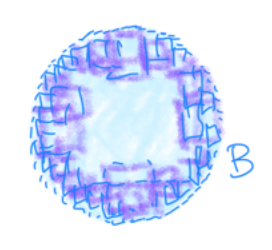
\includegraphics[scale=0.3]{images/base_rn} 
    \end{center}
    Sin embargo, la base de abiertos lo sigue siendo si escogemos otra norma en $\mathbb{R}^n$ distinta de la euclídea, puesto que estas normas eran equivalentes en $\mathbb{R}^n$ (o visto geométricamente, cada bola de una norma contiene otra más pequeña de otra norma distinta y viceversa)
    \begin{center}
        
\includegraphics[scale=0.3]{images/bases_alternativas_rn} 
    \end{center}
    porque
    \[
    B\left( x, \varepsilon \right) = \bigcup_{i \in  I} cuadrados = \bigcup_{j \in J} rectangulos
    \]
\end{enumerate}
\end{ej}

\begin{pg}
    Como antes, a menudo basta considerar los abiertos de $\mathcal{B}$ 
\end{pg}

\begin{il}
$A \subset X$ denso $\Leftrightarrow \forall B \in \mathcal{B}, B \cap A \neq \emptyset$.
\end{il}

\begin{prop}
Sea $X$ un conjunto de puntos y $\mathcal{B} := {B_i}_{i\in I} \subset \mathcal{P}\left( X \right)$ una colección de subconjuntos, esta colección define una topología $\mathcal{T}$ única en $X$ si y sólo si: 
\begin{itemize}
    \item $X = \bigcup_{i\in I} B_i$.
    \item $\forall B_i,B_j\in \mathcal{B} \mbox{ y } \forall x \in B_i \cap B_j, \ \exists B_k \in \mathcal{B} : x\in B_k\subset B_i \cap B_j$.
\end{itemize}
%TODO: Fix imagen
\begin{center}
    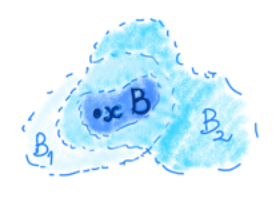
\includegraphics[scale=0.3]{images/base_unica} 
\end{center}
\end{prop}
%TODO: Mejorar
\begin{demo}
\begin{itemize}
\item $\Rightarrow$

Trivial por las propiedades vistas sobre topología.

\item $\Leftarrow$

Veamos que se verifican las condiciones sobre la topología:
\begin{itemize}
    \item \textbf{Unicidad}: $\mathcal{T} = \{\bigcup_{i \in  I} B_i: \{B_i\} \subset \mathcal{B}\}$.
    \item \textbf{Existencia}: Esa $\mathcal{T}$ es efectivamente topología. 
        \begin{itemize}
            \item $\emptyset \in \mathcal{T}$, $X = \bigcup_{i\in I} B_i \in \mathcal{T}$.
            \item Uniones: $\bigcup_{j\in J} \left(\bigcup_{i\in I} B_{i}\right) = \bigcup_{j\in J} B_{ij} \in \mathcal{T}$. 
            \item Intersecciones finitas: $B_1, B_2 \in \mathcal{B} \Rightarrow B_1 \cap B_2 = \bigcup_{x \in B_1 \cap B_2} B^x \in \mathcal{T}$.
            $$
            x \in \left( \bigcup_{i} B_i \right) \cap \left( \bigcup_{k} B_k \right) \Rightarrow x \in B_{i_0} \cap B_{k_0} \Rightarrow \exists B^x \in \mathcal{B} : x\in B^x \subset B_{i_0} \cap B_{k_0}
            $$
            Por tanto, podemos decir que $\left( \bigcup_{i} B_i \right) \cap \left( \bigcup_{k} B_k \right) = \bigcup_{x} B^x \in \mathcal{T}
            $ y se tiene el resultado.
        \end{itemize}
\end{itemize}
\end{itemize}
\end{demo}

\section{Topología relativa}%
\label{sec:topologia_relativa}
\begin{defi}[Topología Relativa]
Sea $\left( X, \mathcal{T} \right)$ un espacio topológico e $Y \subset X$ un subconjunto de puntos, definimos la \textbf{topología relativa\footnote{La comprobación de que efectivamente se trata de una topología es completamente trivial.} en $Y$} como
$$
\mathcal{T}|_Y = \{U \cap Y: U \in \mathcal{T}\}
$$
Además, decimos que $\left( Y, \mathcal{T}|_Y \right)$ es un \textbf{subespacio} de $\left( X, \mathcal{T} \right)$ y que $\left( X, \mathcal{T} \right)$ es el espacio \textbf{ambiente}. 
\begin{center}
    %TODO: Fix imagen
    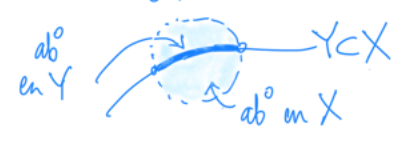
\includegraphics[scale=0.3]{images/def_subespacio_top} 
\end{center}
\end{defi}

\begin{obs}
\begin{enumerate}
    \item Los cerrados de la topología relativa $\mathcal{T}|_Y$ son la intersección $F\cap Y$ de $Y$ con cerrados $F$ en $\mathcal{T}$.
    $$
    F \stackrel{cerr}{\subset} Y \Rightarrow F = Y\setminus W : W \stackrel{ab}{\subset} Y \Rightarrow \exists U \stackrel{ab}{\subset}X : Y\cap U = W \Rightarrow F = Y \setminus (Y \cap U) = Y \cap  (X\setminus U) = Y \cap F_x : F_x \stackrel{cerr}{\subset} X
    $$
    \item Si tenemos una base $\mathcal{V}^a$ de entornos en el espacio ambiente $(X,\mathcal{T})$, la base de entornos en el subespacio $(Y,\mathcal{T}\mid_Y)$ se obtiene intersecando los elementos de la base ambiente con el subespacio, es decir, $\mathcal{V}^a_Y := \mathcal{V}^a \cap Y := \{V^a \cap Y : V^a \in \mathcal{V}^a\}$.

    \item Si tenemos una base $\mathcal{B}$ de abiertos en el espacio ambiente $(X,\mathcal{T})$, la base de abiertos en el subespacio $(Y,\mathcal{T}\mid_Y)$ se obtiene intersecando\footnote{Esta idea suele ser general, las construcciones en los subespacios se hacen intersecando elementos del espacio ambiente con el subespacio.} los elementos de la base ambiente con el subespacio, es decir, $\mathcal{B}_Y := \mathcal{B} \cap Y := \{B \cap Y : B \in \mathcal{B}\}$.
\end{enumerate}
\end{obs}


\begin{ej}
\begin{enumerate}
    \item Si $y$ es un punto aislado de $Y$, por la definición que hemos dado de la topología relativa, su topología relativa sería $\mathcal{T}|_Y := \{ U \cap \{y\} \} = \{y\}$. Por tanto, es abierto en su topología.
    
    \item Retomando el ejemplo anterior, si todos los puntos de $Y$ son aislados, hemos visto que todos son abiertos (pues cortar un abierto con ellos da ellos mismos) y, por tanto, la topología $\mathcal{T}\mid_Y $ es la discreta. Por ejemplo, en $\mathbb{Z} \subset \mathbb{R}$:
    %TODO: Fix imagen
    \begin{center}
        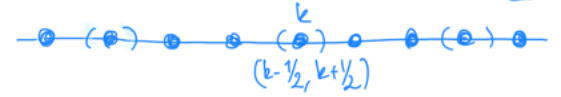
\includegraphics[scale=0.3]{images/def_subespacio_discreto} 
    \end{center}

    \item Si tomamos la topología del punto $(a \in X, \mathcal{T}_a|_{X \setminus \{a\}})$ vemos que se trata de la discreta.
\end{enumerate}
\end{ej}

\begin{obs}
\begin{enumerate}
    \item Los abiertos $W$ de un subespacio abierto $Y \stackrel{ab}{\subset} X$ son abiertos en el espacio ambiente $X$.
   	$$
    W = U \cap Y : U,Y\stackrel{ab}{\subset} X \Rightarrow W \stackrel{ab}{\subset} X 
    $$
    \item Los cerrados $F$ de un subespacio cerrado $Y \stackrel{cerr}{\subset} X$ son cerrados en el espacio ambiente $X$.
    $$
    F = C \cap Y : Y,C\stackrel{cerr}{\subset} X \Rightarrow F \stackrel{cerr}{\subset} X
    $$
\end{enumerate}
\end{obs}

